\section{opttritri.h File Reference}
\label{opttritri_8h}\index{opttritri.h@{opttritri.h}}
{\tt \#include $<$math.h$>$}\par
{\tt \#include \char`\"{}meshmorph.h\char`\"{}}\par


Include dependency graph for opttritri.h:\begin{figure}[H]
\begin{center}
\leavevmode
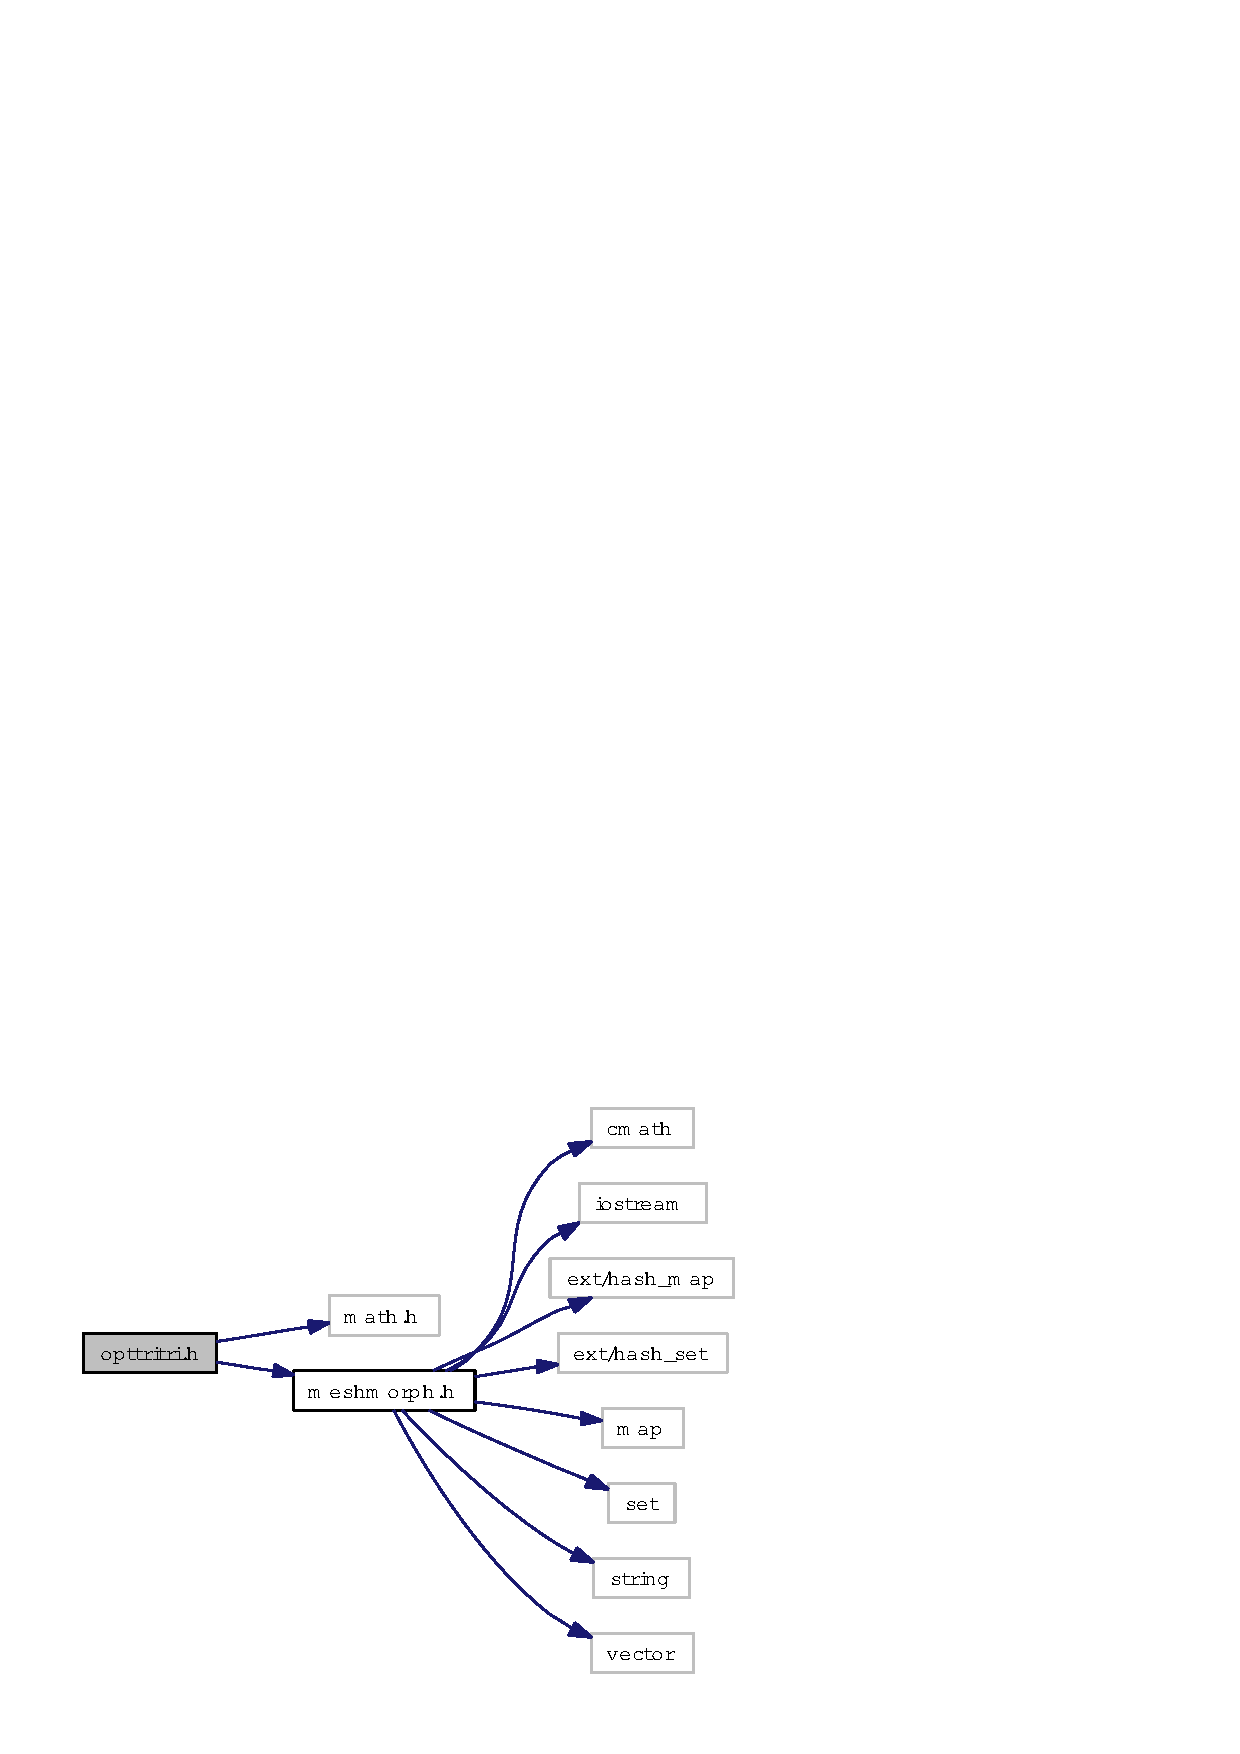
\includegraphics[width=178pt]{opttritri_8h__incl}
\end{center}
\end{figure}


This graph shows which files directly or indirectly include this file:\begin{figure}[H]
\begin{center}
\leavevmode
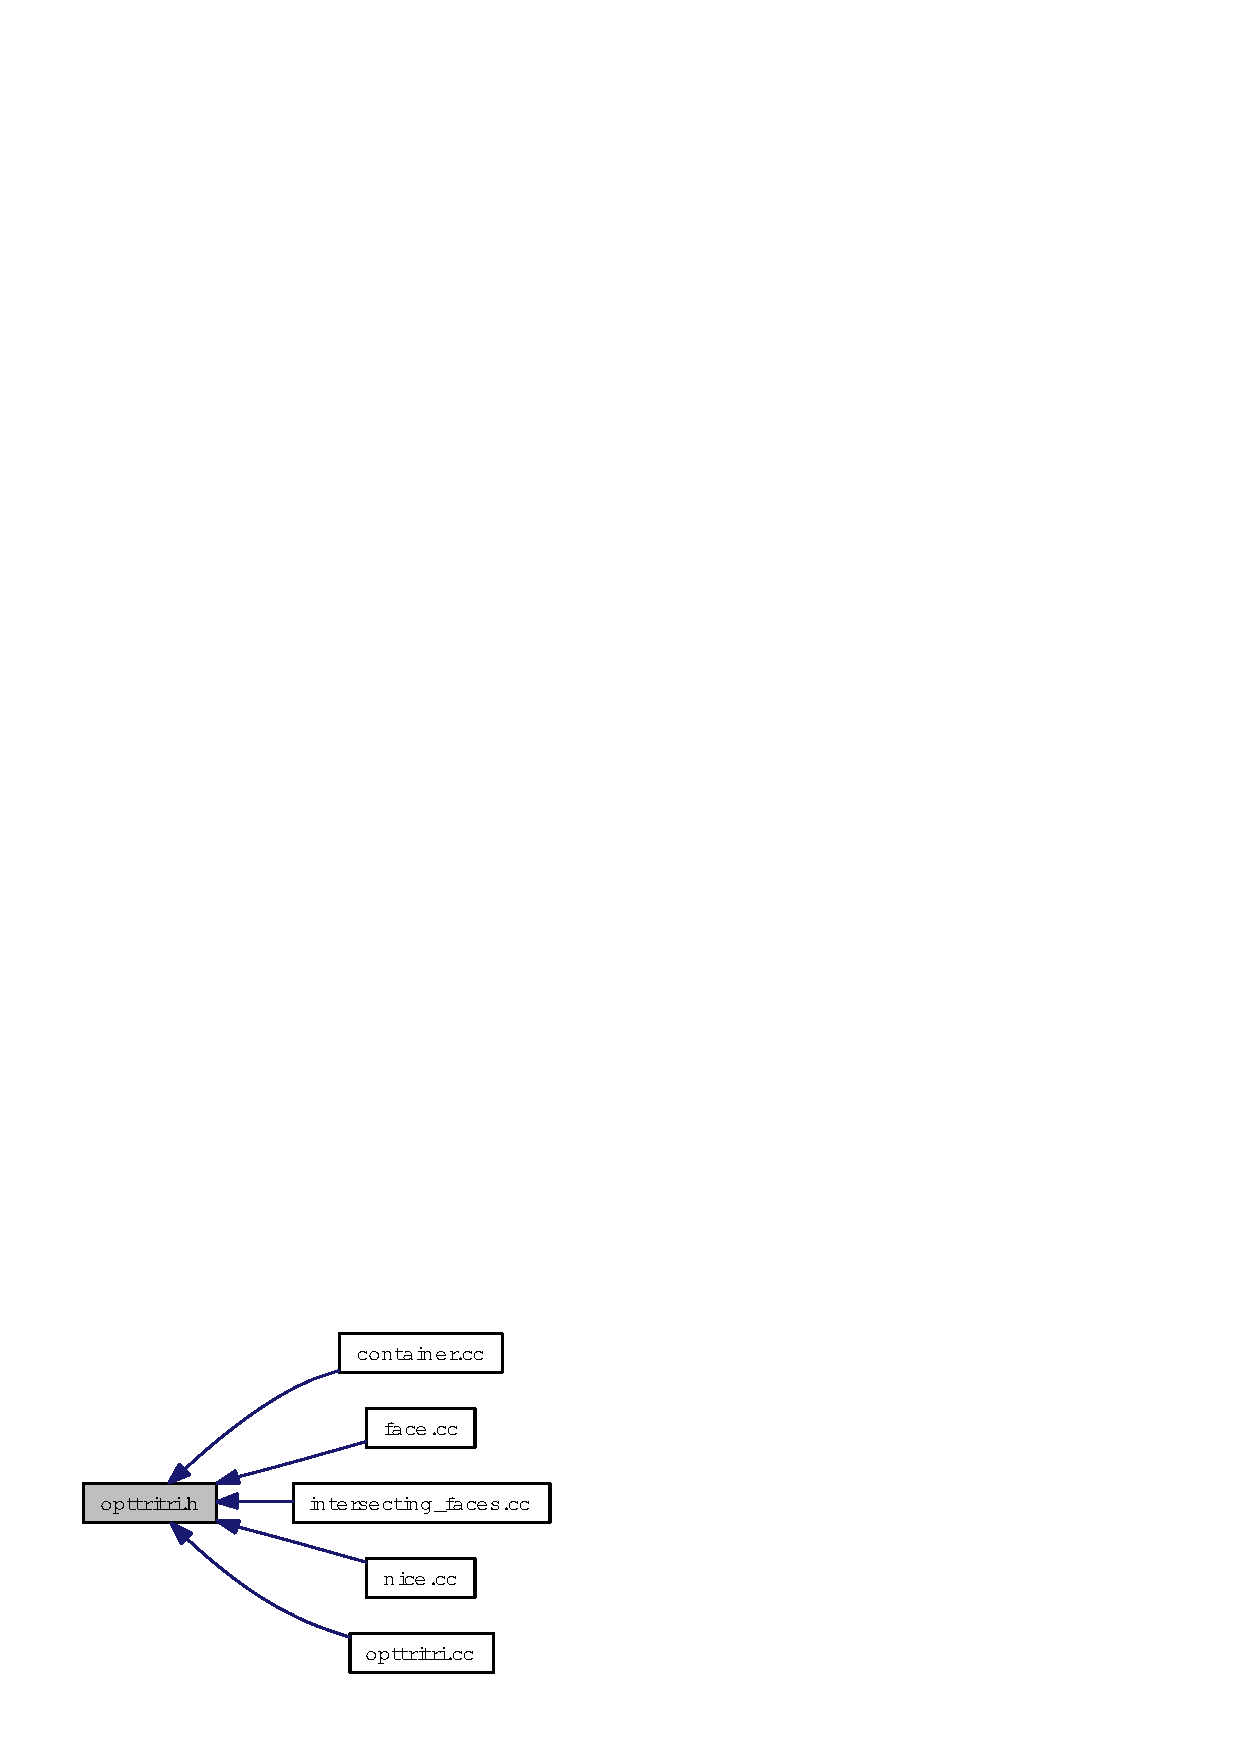
\includegraphics[width=134pt]{opttritri_8h__dep__incl}
\end{center}
\end{figure}
\subsection*{Defines}
\begin{CompactItemize}
\item 
\#define {\bf FABS}(x)~(fabs(x))
\item 
\#define {\bf USE\_\-EPSILON\_\-TEST}~TRUE
\item 
\#define {\bf SORT}(a, b)
\item 
\#define {\bf EDGE\_\-EDGE\_\-TEST}(V0, U0, U1)
\item 
\#define {\bf EDGE\_\-AGAINST\_\-TRI\_\-EDGES}(V0, V1, U0, U1, U2)
\item 
\#define {\bf POINT\_\-IN\_\-TRI}(V0, U0, U1, U2)
\item 
\#define {\bf NEWCOMPUTE\_\-INTERVALS}(VV0, VV1, VV2, D0, D1, D2, D0D1, D0D2, A, B, C, X0, X1)
\end{CompactItemize}
\subsection*{Functions}
\begin{CompactItemize}
\item 
int {\bf coplanar\_\-tri\_\-tri} ({\bf vector3} \&N, {\bf vector3} const $\ast$V0, {\bf vector3} const $\ast$V1, {\bf vector3} const $\ast$V2, {\bf vector3} const $\ast$U0, {\bf vector3} const $\ast$U1, {\bf vector3} const $\ast$U2)
\item 
int {\bf No\-Div\-Tri\-Tri\-Isect} ({\bf vector3} const $\ast$V0, {\bf vector3} const $\ast$V1, {\bf vector3} const $\ast$V2, {\bf vector3} const $\ast$U0, {\bf vector3} const $\ast$U1, {\bf vector3} const $\ast$U2)
\item 
int {\bf intersect\_\-triangle3} ({\bf vector3} const $\ast$orig, {\bf vector3} const $\ast$end, {\bf vector3} const $\ast$normal, {\bf vector3} const $\ast$vert0, {\bf vector3} const $\ast$vert1, {\bf vector3} const $\ast$vert2, {\bf result} \&r)
\end{CompactItemize}


\subsection{Define Documentation}
\index{opttritri.h@{opttritri.h}!EDGE_AGAINST_TRI_EDGES@{EDGE\_\-AGAINST\_\-TRI\_\-EDGES}}
\index{EDGE_AGAINST_TRI_EDGES@{EDGE\_\-AGAINST\_\-TRI\_\-EDGES}!opttritri.h@{opttritri.h}}
\subsubsection{\setlength{\rightskip}{0pt plus 5cm}\#define EDGE\_\-AGAINST\_\-TRI\_\-EDGES(V0, V1, U0, U1, U2)}\label{opttritri_8h_831bfa37e6247abd79136fbd5c5ebee3}


\textbf{Value:}

\begin{Code}\begin{verbatim}{                                              \
  double Ax,Ay,Bx,By,Cx,Cy,e,d,f;               \
  Ax=V1->p[i0]-V0->p[i0];                            \
  Ay=V1->p[i1]-V0->p[i1];                            \
  /* test edge U0,U1 against V0,V1 */          \
  EDGE_EDGE_TEST(V0,U0,U1);                    \
  /* test edge U1,U2 against V0,V1 */          \
  EDGE_EDGE_TEST(V0,U1,U2);                    \
  /* test edge U2,U1 against V0,V1 */          \
  EDGE_EDGE_TEST(V0,U2,U0);                    \
}
\end{verbatim}\end{Code}
\index{opttritri.h@{opttritri.h}!EDGE_EDGE_TEST@{EDGE\_\-EDGE\_\-TEST}}
\index{EDGE_EDGE_TEST@{EDGE\_\-EDGE\_\-TEST}!opttritri.h@{opttritri.h}}
\subsubsection{\setlength{\rightskip}{0pt plus 5cm}\#define EDGE\_\-EDGE\_\-TEST(V0, U0, U1)}\label{opttritri_8h_1c2f23f22443903c367825ed07f65c0f}


\textbf{Value:}

\begin{Code}\begin{verbatim}Bx=U0->p[i0]-U1->p[i0];                                   \
By=U0->p[i1]-U1->p[i1];                                   \
Cx=V0->p[i0]-U0->p[i0];                                   \
Cy=V0->p[i1]-U0->p[i1];                                   \
f=Ay*Bx-Ax*By;                                      \
d=By*Cx-Bx*Cy;                                      \
if((f>0 && d>=0 && d<=f) || (f<0 && d<=0 && d>=f))  \
{                                                   \
  e=Ax*Cy-Ay*Cx;                                    \
  if(f>0)                                           \
  {                                                 \
    if(e>=0 && e<=f) return 1;                      \
  }                                                 \
  else                                              \
  {                                                 \
    if(e<=0 && e>=f) return 1;                      \
  }                                                 \
}
\end{verbatim}\end{Code}
\index{opttritri.h@{opttritri.h}!FABS@{FABS}}
\index{FABS@{FABS}!opttritri.h@{opttritri.h}}
\subsubsection{\setlength{\rightskip}{0pt plus 5cm}\#define FABS(x)~(fabs(x))}\label{opttritri_8h_9b649f4d878e64a80b4cd2cad45f43b3}


\index{opttritri.h@{opttritri.h}!NEWCOMPUTE_INTERVALS@{NEWCOMPUTE\_\-INTERVALS}}
\index{NEWCOMPUTE_INTERVALS@{NEWCOMPUTE\_\-INTERVALS}!opttritri.h@{opttritri.h}}
\subsubsection{\setlength{\rightskip}{0pt plus 5cm}\#define NEWCOMPUTE\_\-INTERVALS(VV0, VV1, VV2, D0, D1, D2, D0D1, D0D2, A, B, C, X0, X1)}\label{opttritri_8h_6fec81c12c0221d10380595bb646bc65}


\index{opttritri.h@{opttritri.h}!POINT_IN_TRI@{POINT\_\-IN\_\-TRI}}
\index{POINT_IN_TRI@{POINT\_\-IN\_\-TRI}!opttritri.h@{opttritri.h}}
\subsubsection{\setlength{\rightskip}{0pt plus 5cm}\#define POINT\_\-IN\_\-TRI(V0, U0, U1, U2)}\label{opttritri_8h_dd43cd9d9b223e41583e509300913a33}


\textbf{Value:}

\begin{Code}\begin{verbatim}{                                           \
  double a,b,c,d0,d1,d2;                     \
  /* is T1 completly inside T2? */          \
  /* check if V0 is inside tri(U0,U1,U2) */ \
  a=U1->p[i1]-U0->p[i1];                          \
  b=-(U1->p[i0]-U0->p[i0]);                       \
  c=-a*U0->p[i0]-b*U0->p[i1];                     \
  d0=a*V0->p[i0]+b*V0->p[i1]+c;                   \
  \
  a=U2->p[i1]-U1->p[i1];                          \
  b=-(U2->p[i0]-U1->p[i0]);                       \
  c=-a*U1->p[i0]-b*U1->p[i1];                     \
  d1=a*V0->p[i0]+b*V0->p[i1]+c;                   \
  \
  a=U0->p[i1]-U2->p[i1];                          \
  b=-(U0->p[i0]-U2->p[i0]);                       \
  c=-a*U2->p[i0]-b*U2->p[i1];                     \
  d2=a*V0->p[i0]+b*V0->p[i1]+c;                   \
  if(d0*d1>0.0)                             \
  {                                         \
    if(d0*d2>0.0) return 1;                 \
  }                                         \
}
\end{verbatim}\end{Code}
\index{opttritri.h@{opttritri.h}!SORT@{SORT}}
\index{SORT@{SORT}!opttritri.h@{opttritri.h}}
\subsubsection{\setlength{\rightskip}{0pt plus 5cm}\#define SORT(a, b)}\label{opttritri_8h_c226bc1ed04fd7d4865263484ed22a47}


\textbf{Value:}

\begin{Code}\begin{verbatim}if(a>b)    \
{          \
  double c; \
  c=a;     \
  a=b;     \
  b=c;     \
}
\end{verbatim}\end{Code}
\index{opttritri.h@{opttritri.h}!USE_EPSILON_TEST@{USE\_\-EPSILON\_\-TEST}}
\index{USE_EPSILON_TEST@{USE\_\-EPSILON\_\-TEST}!opttritri.h@{opttritri.h}}
\subsubsection{\setlength{\rightskip}{0pt plus 5cm}\#define USE\_\-EPSILON\_\-TEST~TRUE}\label{opttritri_8h_30e72ae9306395819bee85199878fa9e}




\subsection{Function Documentation}
\index{opttritri.h@{opttritri.h}!coplanar_tri_tri@{coplanar\_\-tri\_\-tri}}
\index{coplanar_tri_tri@{coplanar\_\-tri\_\-tri}!opttritri.h@{opttritri.h}}
\subsubsection{\setlength{\rightskip}{0pt plus 5cm}int coplanar\_\-tri\_\-tri ({\bf vector3} \& {\em N}, {\bf vector3} const $\ast$ {\em V0}, {\bf vector3} const $\ast$ {\em V1}, {\bf vector3} const $\ast$ {\em V2}, {\bf vector3} const $\ast$ {\em U0}, {\bf vector3} const $\ast$ {\em U1}, {\bf vector3} const $\ast$ {\em U2})}\label{opttritri_8h_7cc10013bc791c2bfab4bb52a1a2809e}


Determine whether two coplanar triangles intersect. \begin{Desc}
\item[Parameters:]
\begin{description}
\item[\mbox{$\leftarrow$} {\em N}]Not sure what this is. \item[\mbox{$\leftarrow$} {\em V0}]First vertex of first triangle. \item[\mbox{$\leftarrow$} {\em V1}]second vertex of first triangle. \item[\mbox{$\leftarrow$} {\em V2}]Third vertex of first triangle. \item[\mbox{$\leftarrow$} {\em U0}]First vertex of second triangle. \item[\mbox{$\leftarrow$} {\em U1}]second vertex of second triangle. \item[\mbox{$\leftarrow$} {\em U2}]Third vertex of second triangle. \end{description}
\end{Desc}
\begin{Desc}
\item[Returns:]1 if triangles intersect; 0 otherwise. \end{Desc}
\index{opttritri.h@{opttritri.h}!intersect_triangle3@{intersect\_\-triangle3}}
\index{intersect_triangle3@{intersect\_\-triangle3}!opttritri.h@{opttritri.h}}
\subsubsection{\setlength{\rightskip}{0pt plus 5cm}int intersect\_\-triangle3 ({\bf vector3} const $\ast$ {\em orig}, {\bf vector3} const $\ast$ {\em end}, {\bf vector3} const $\ast$ {\em normal}, {\bf vector3} const $\ast$ {\em vert0}, {\bf vector3} const $\ast$ {\em vert1}, {\bf vector3} const $\ast$ {\em vert2}, {\bf result} \& {\em r})}\label{opttritri_8h_d7a9482aa12886f663ad07d306fe8ccb}


Determine if line segment and triangle intersect. \begin{Desc}
\item[Parameters:]
\begin{description}
\item[\mbox{$\leftarrow$} {\em orig}]One end of line segment. \item[\mbox{$\leftarrow$} {\em end}]Other end of line segment. \item[\mbox{$\leftarrow$} {\em normal}]Normal vector of triangle. \item[\mbox{$\leftarrow$} {\em vert0}]First vertex of triangle. \item[\mbox{$\leftarrow$} {\em vert1}]second vertex of triangle. \item[\mbox{$\leftarrow$} {\em vert2}]Third vertex of triangle. \item[\mbox{$\rightarrow$} {\em r}]Record whether line intersects triange along line segment; whether line intersects triangle; and whether line intersects edge of triangle. \end{description}
\end{Desc}
\begin{Desc}
\item[Returns:]1 if triangles intersect; 0 otherwise. \end{Desc}
\index{opttritri.h@{opttritri.h}!NoDivTriTriIsect@{NoDivTriTriIsect}}
\index{NoDivTriTriIsect@{NoDivTriTriIsect}!opttritri.h@{opttritri.h}}
\subsubsection{\setlength{\rightskip}{0pt plus 5cm}int No\-Div\-Tri\-Tri\-Isect ({\bf vector3} const $\ast$ {\em V0}, {\bf vector3} const $\ast$ {\em V1}, {\bf vector3} const $\ast$ {\em V2}, {\bf vector3} const $\ast$ {\em U0}, {\bf vector3} const $\ast$ {\em U1}, {\bf vector3} const $\ast$ {\em U2})}\label{opttritri_8h_964292b46316fc46d2be9ca9570deb64}


Determine whether two triangles intersect. \begin{Desc}
\item[Parameters:]
\begin{description}
\item[\mbox{$\leftarrow$} {\em V0}]First vertex of first triangle. \item[\mbox{$\leftarrow$} {\em V1}]second vertex of first triangle. \item[\mbox{$\leftarrow$} {\em V2}]Third vertex of first triangle. \item[\mbox{$\leftarrow$} {\em U0}]First vertex of second triangle. \item[\mbox{$\leftarrow$} {\em U1}]second vertex of second triangle. \item[\mbox{$\leftarrow$} {\em U2}]Third vertex of second triangle. \end{description}
\end{Desc}
\begin{Desc}
\item[Returns:]1 if triangles intersect; 0 otherwise. \end{Desc}
